\chapter{Экспериментальный раздел}
В текущем разделе будет поставлена цель эксперимента, проведён сам эксперимент и сделаны соответствующие выводы. 

\section{Технические характеристики}

Технические характеристики устройства, на котором выполнялось тестирование, следующие.

\begin{itemize}
	\item Операционная система: Arch Linux \cite{oswind} x86\_64.
	\item Память: 48 GiB.
	\item 4 физических ядра и 8 логических ядра.
	\item процессор: AMD Ryzen 7 3700X 8-Core Processor (16 ядер);
	\item видеокарта: Nvidia GeForce GTX 1080 (8 Гб, 2560 Cuda ядер, 20 SM по 128 Cuda ядер).
\end{itemize}

Тестирование проводилось на компьютере, включенном в сеть электропитания. Во время тестирования ноутбук был нагружен только встроенными приложениями окружения, а также непосредственно системой тестирования.


\section{Постановка эксперимента 1} 

Цель эксперимента -- узнать зависимость количества времени на обработку кадра от количества потоков.

Гипотеза - чем больше потоков, тем лучше. При этом отключена всякая параллельность задач на видеокарте, разговор идет только про количество потоков запуска функции.

На рисунке \ref{img:e4} приведен график зависимости количества миллисекунд от количества потоков.

При количестве потоков <= 9 графический ускоритель начинает цокать.

\begin{figure}[H]
	\begin{center}
		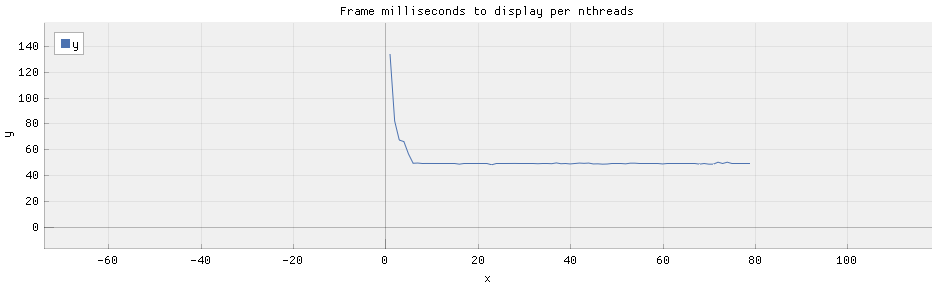
\includegraphics[scale=0.60]{img/avg_time_focused.png}
	\end{center}
	\captionsetup{justification=centering}
	\caption{Зависимость количества миллисекунд (по y) от количества потоков (по x). }
	\label{img:e4}
\end{figure}


\section{Постановка эксперимента 2} 

Цель эксперимента -- узнать зависимость количества времени на обработку кадра от расстояния до объекта.

Гипотеза, че ближе объект, тем больше времени на обработку кадра. Это связано с разной площадью граней.
Решить проблему может виртуальная геометрия. В ходе эксперимента был убран порог на максимальную площадь ребра, о чем свидетельствовали
артефакты при близости объекта.

На таблице \ref{tbl:virt_geom} приведены замеры времени отрисовки кадра в зависимости от расстояния до объекта.

Рисунок \ref{img:vgeom_graph} показывает эту зависимость графически. 

\begin{table}[H]
	\centering
	\begin{center}
		\begin{threeparttable}
		\caption{Зависимость времени на кадр от расстояния до объекта и от использования виртуальной геометрии. }
		\label{tbl:virt_geom}
			\centering
			\begin{tabular}{ |P{0.3\linewidth}|P{0.3\linewidth}|P{0.3\linewidth}| }
			\toprule
			Евклидово расстояние до центра объекта (у.е.) & Время отрисовки кадра (ms) & Виртуальная геометрия \\
			\midrule
			7                                             & 16                         & Включена             \\
			7                                             & 17                         & Выключена             \\
			6                                             & 33                         & Выключена             \\
			6                                             & 16                         & Включена              \\
			5.4                                           & 33                         & Выключена             \\
			5.4                                           & 15                         & Включена              \\
			4.8                                           & 49                         & Выключена             \\ 
			4.8                                           & 16                         & Включена              \\
			\bottomrule
			\end{tabular}
		\end{threeparttable}
	\end{center}
\end{table}

\begin{figure}[H]
	\begin{center}
		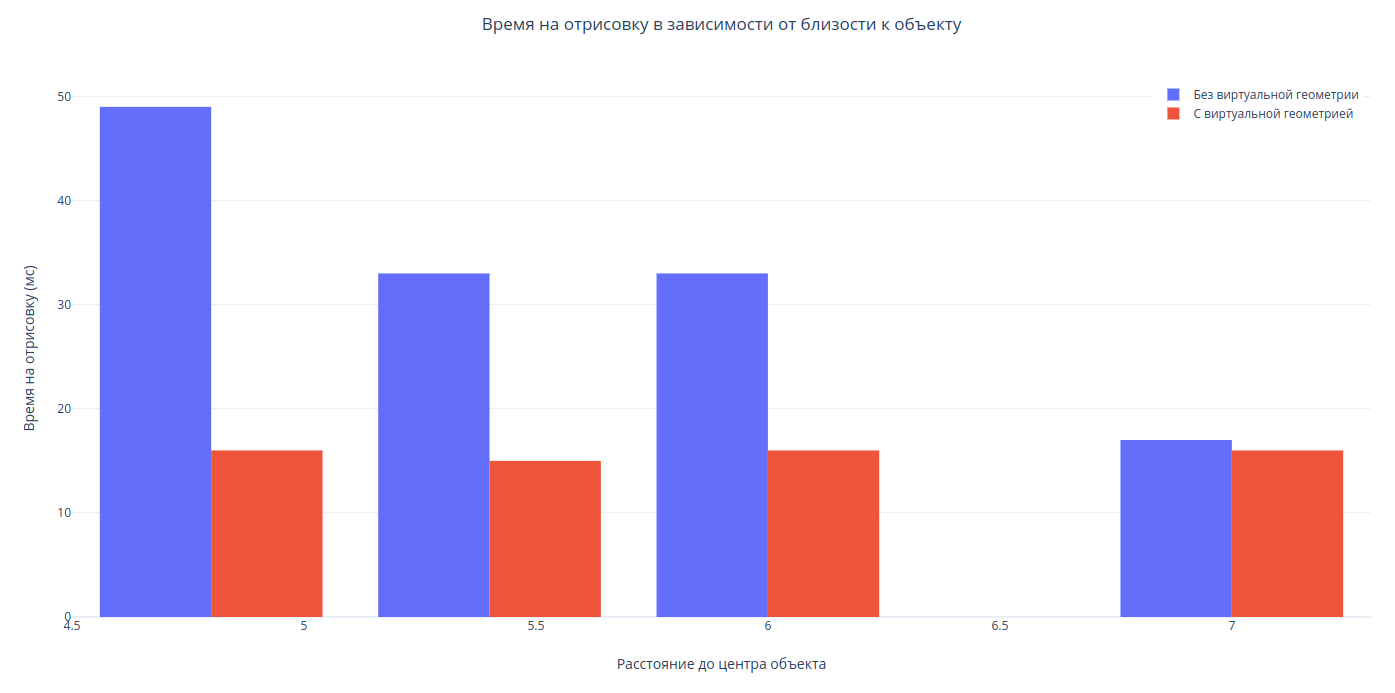
\includegraphics[scale=0.4]{img/vgeom_graph.png}
	\end{center}
	\captionsetup{justification=centering}
	\caption{Зависимость количества миллисекунд на кадр от близости объекта.}
	\label{img:vgeom_graph}
\end{figure}

Можно сделать вывод о том, что неравенство площадей существенно и негативно влияет на производительность вблизи объекта, а устранить эту проблему помогает использование виртуальной геометрии.

\section{Постановка эксперимента 3} 

Цель эксперимента -- узнать зависимость количества времени на обработку кадра количества отрисовываемых объектов и от куллига по пирамиде видимости.

Гипотеза - программа высоко параллельна и количество миллисекунд на обработку кадра зависит от количества объектов нелинейно.

\begin{table}[H]
	\centering
	\begin{center}
		\begin{threeparttable}
		\caption{Зависимость времени на кадр от расстояния до объекта и от использования виртуальной геометрии. }
		\label{tbl:virt_geom}
			\centering
			\begin{tabular}{ |P{0.25\linewidth}|P{0.2\linewidth}|P{0.25\linewidth}|P{0.25\linewidth}| }
			\toprule
			Количество объектов на сцене & Время отрисовки кадра (ms) & Frustum Culling & Количество объектов после фильтрации \\
			\midrule
1                            & 15                         & Выключен & 1                                    \\
			1                            & 15                         & Включен  & 1                                    \\
100                          & 16                         & Выключен  & 100                                  \\
100                          & 16                         & Включен  & 80                                   \\
1000                         & 24                         & Выключен & 1000                                 \\
1000                         & 16                         & Включен  & 200                                  \\
10000                        & 55                         & Выключен & 10000                                \\
10000                        & 28                         & Включен  & 1500                                 \\

			\bottomrule
			\end{tabular}
		\end{threeparttable}
	\end{center}
\end{table}

\section*{Вывод}

В результате эксперимента было выявлено, что оптимизированный алгоритм обратной трассировки лучей на самом деле дает выигрыш во времени, так как требует меньшего количества лучей для построения сцены. Кроме того, расчитанные аналитическим способом результаты были подтверждены на практике.

